\section{Atividades}

\subsection{Atividade 1 -- Campanha de Phishing com SET}

\begin{figure}[H]
    \centering
    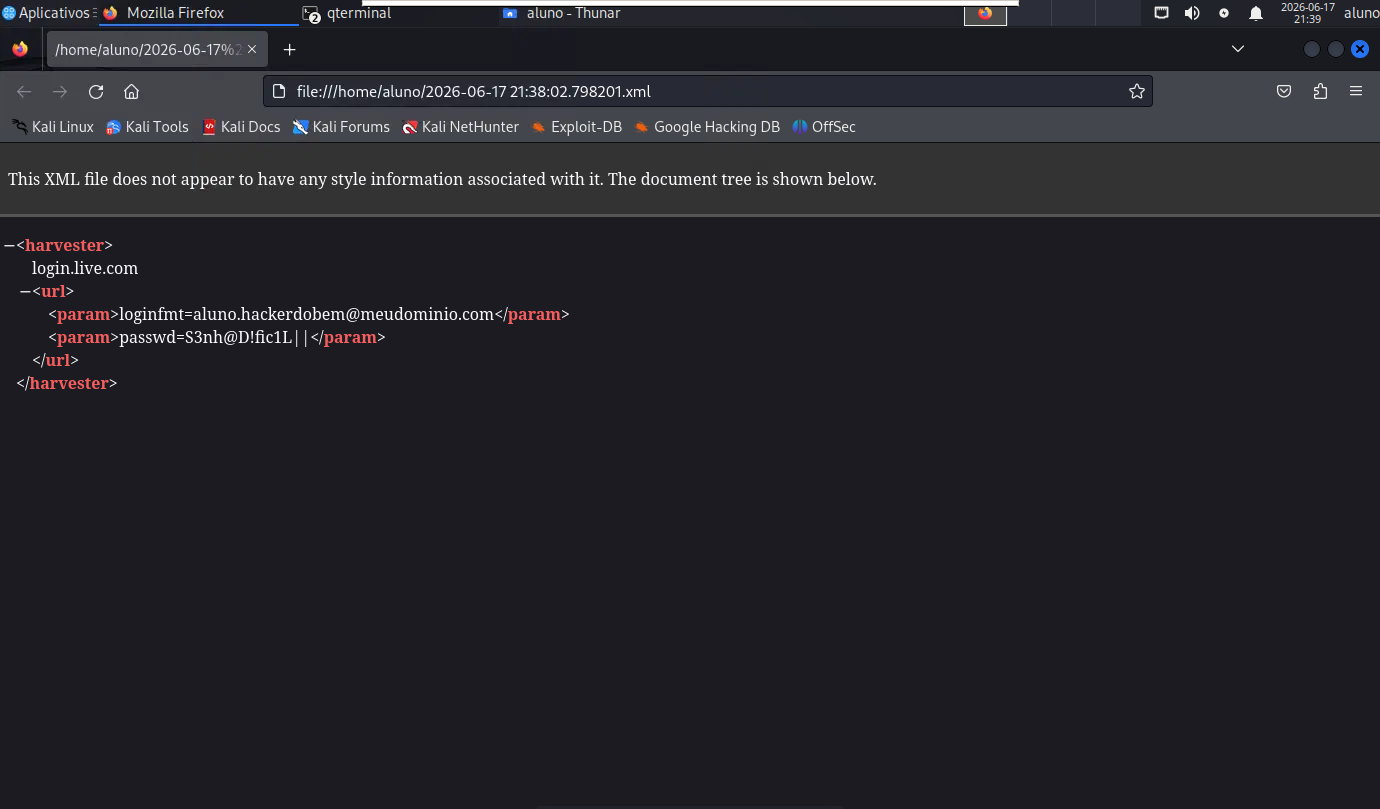
\includegraphics[width=0.95\textwidth]{./fig/atividade1-set.png}
    \caption{Execução da campanha de phishing utilizando SET.}
\end{figure}

\paragraph{}
Foi utilizada a ferramenta Social Engineering Toolkit (SET) para criação de uma
página falsa de autenticação baseada no Office365. O objetivo foi demonstrar a
captura de credenciais em um cenário controlado de engenharia social.

\subsection{Atividade 2 -- Campanha de Phishing com Gophish}

\begin{figure}[H]
    \centering
    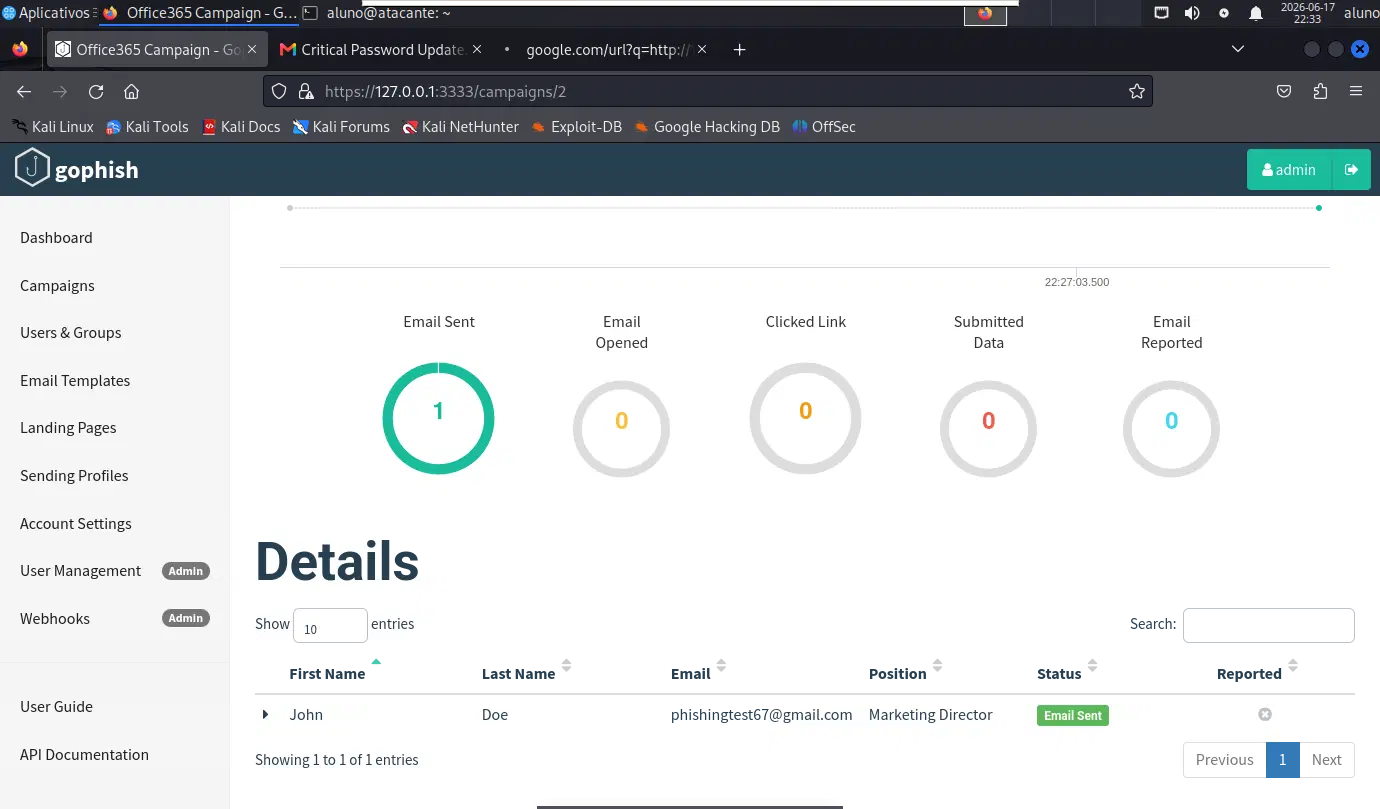
\includegraphics[width=0.95\textwidth]{./fig/atividade2-gophish.png}
    \caption{Campanha criada e monitorada através do Gophish.}
\end{figure}

\paragraph{}
Foi criada uma campanha de phishing utilizando a plataforma Gophish, incluindo
template de e-mail, página de destino e acompanhamento dos eventos gerados
durante a interação do usuário com a campanha.

\subsection{Atividade 3 -- Exploração com BeEF}

\begin{figure}[H]
    \centering
    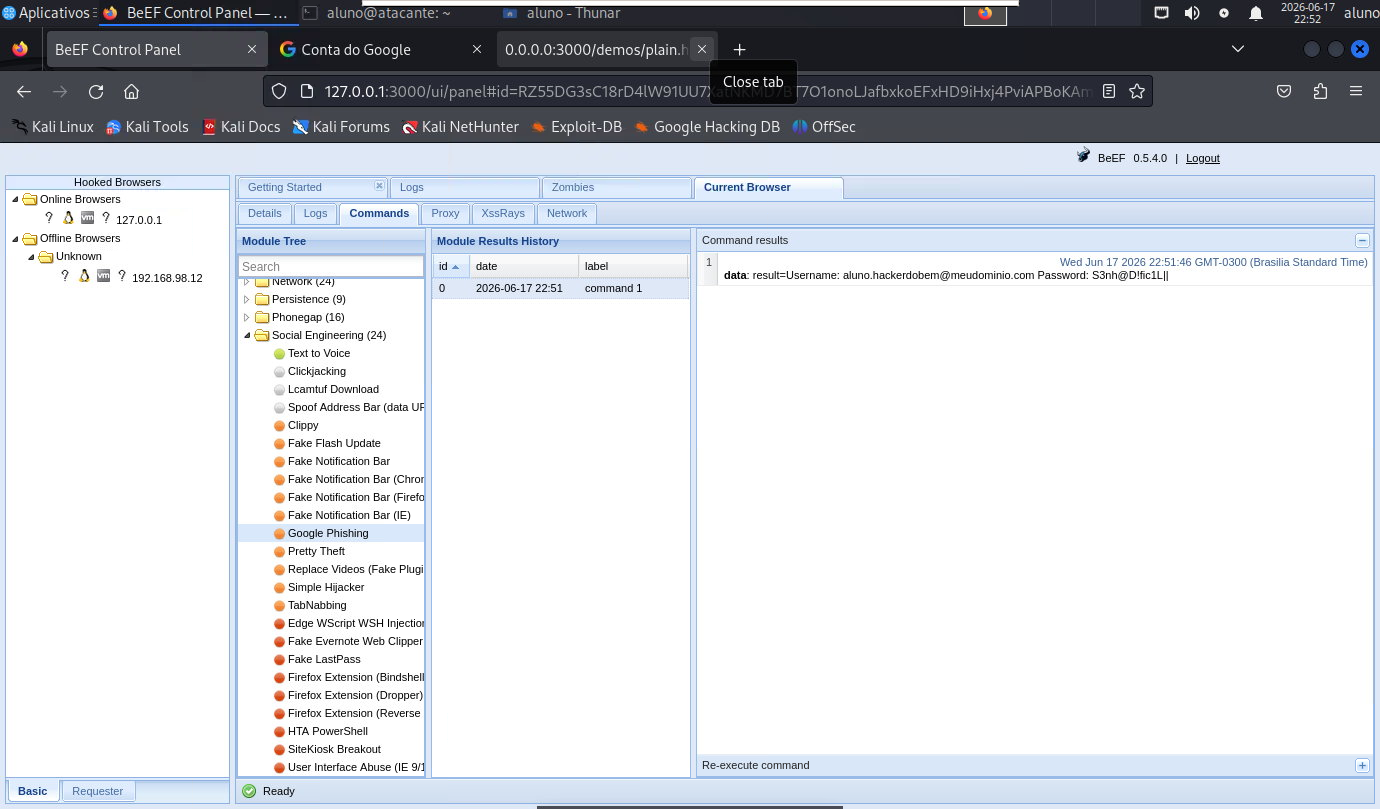
\includegraphics[width=0.95\textwidth]{./fig/atividade3-beef.png}
    \caption{Execução de ações utilizando o framework BeEF.}
\end{figure}

\paragraph{}
Foi utilizado o Browser Exploitation Framework (BeEF) para demonstrar técnicas
de interação com navegadores comprometidos em ambiente de laboratório,
evidenciando riscos associados à execução de conteúdo malicioso em sessões
ativas de usuários.

\subsection{Atividade 4 -- Análise e Mitigação de Riscos}

\paragraph{}
A análise das campanhas simuladas de phishing demonstrou que técnicas de
engenharia social podem induzir usuários a fornecer credenciais, acessar links
maliciosos ou executar ações que comprometam a segurança da organização.

\paragraph{}
Os principais riscos identificados foram:

\begin{itemize}
    \item Exposição de credenciais corporativas;
    \item Acesso não autorizado a sistemas internos;
    \item Comprometimento de contas de usuário;
    \item Vazamento de informações confidenciais;
    \item Possível disseminação de malware;
    \item Movimentação lateral dentro da rede corporativa.
\end{itemize}

\paragraph{}
Os riscos foram priorizados conforme sua gravidade e impacto potencial:

\begin{itemize}
    \item \textbf{Alta prioridade:} exposição de credenciais e acesso não
      autorizado;
    \item \textbf{Média prioridade:} vazamento de informações confidenciais;
    \item \textbf{Média prioridade:} propagação de malware;
    \item \textbf{Baixa prioridade:} impactos operacionais indiretos.
\end{itemize}

\paragraph{}
Para mitigação dos riscos identificados, recomenda-se:

\begin{itemize}
    \item Implementação de autenticação multifator (MFA);
    \item Utilização de filtros antiphishing e proteção de e-mail;
    \item Atualização periódica de sistemas e navegadores;
    \item Monitoramento contínuo de eventos de segurança;
    \item Realização de campanhas periódicas de conscientização;
    \item Aplicação do princípio do menor privilégio;
    \item Implementação de ferramentas EDR e antivírus corporativo.
\end{itemize}

\begin{table}[H]
\centering
\small
\begin{tabular}{|p{5cm}|p{4cm}|p{2.5cm}|}
\hline
\textbf{Ação} & \textbf{Responsável} & \textbf{Prazo} \\
\hline
Implantação de MFA & Equipe de TI & 30 dias \\
\hline
Treinamento de usuários & Segurança da Informação & 60 dias \\
\hline
Atualização dos sistemas & Administração de TI & Contínuo \\
\hline
Monitoramento de eventos & SOC / Equipe de Segurança & Contínuo \\
\hline
\end{tabular}
\caption{Plano de mitigação dos riscos identificados.}
\end{table}

\subsection{Atividade 5 -- Treinamento de Conscientização em Engenharia Social}

\paragraph{}
Com base nos resultados obtidos durante as campanhas simuladas, observou-se que
os principais fatores de risco estão relacionados à confiança excessiva dos
usuários em mensagens aparentemente legítimas e à falta de verificação da
origem das solicitações recebidas.

\paragraph{}
O treinamento de conscientização deve abordar os principais tipos de ataques de
engenharia social:

\begin{itemize}
    \item \textbf{Phishing:} mensagens falsas que buscam capturar credenciais
      ou dados sensíveis;
    \item \textbf{Spear Phishing:} ataques direcionados a pessoas específicas;
    \item \textbf{Pretexting:} criação de uma identidade ou cenário falso para
      obter informações;
    \item \textbf{Baiting:} utilização de recompensas ou arquivos atrativos
      para induzir ações;
    \item \textbf{Vishing:} golpes realizados por telefone;
    \item \textbf{Smishing:} ataques realizados por mensagens SMS.
\end{itemize}

\paragraph{}
Os usuários devem estar atentos aos seguintes sinais de alerta:

\begin{itemize}
    \item Solicitações urgentes ou fora do padrão;
    \item Links encurtados ou suspeitos;
    \item Remetentes desconhecidos;
    \item Erros gramaticais ou de formatação;
    \item Solicitação de senhas ou informações confidenciais.
\end{itemize}

\paragraph{}
Como boas práticas de prevenção, recomenda-se:

\begin{itemize}
    \item Verificar cuidadosamente remetentes e URLs;
    \item Não clicar em links suspeitos;
    \item Confirmar solicitações sensíveis por canais alternativos;
    \item Utilizar senhas fortes e autenticação multifator;
    \item Não compartilhar credenciais;
    \item Reportar imediatamente mensagens suspeitas à equipe de segurança;
    \item Manter sistemas e navegadores atualizados.
\end{itemize}

\paragraph{}
A realização periódica de treinamentos e campanhas simuladas contribui para
reduzir a probabilidade de sucesso de ataques de engenharia social e aumentar a
maturidade de segurança dos usuários.
